\section{Caso de estudio: calentamiento de 24 toneladas de glucosa desde 40~\textdegree C hasta 60~\textdegree C con 14~m\textsuperscript{2} de área de transferencia}
\label{sec:calentamiento_24ton}

El presente caso de estudio evalúa el tiempo requerido para calentar 24~ton de jarabe de glucosa Globe 1130 desde 40~\textdegree C hasta 60~\textdegree C, empleando un sistema de media caña con área de transferencia de 14~m\textsuperscript{2}. La masa seleccionada corresponde a una descarga típica de carrotanque y permite analizar el comportamiento transitorio del sistema cuando opera como unidad de calentamiento independiente. Se evalúan dos temperaturas de agua de calentamiento: 65~\textdegree C y 75~\textdegree C, manteniendo la velocidad del agua en la media caña en 2,5~m/s.

\subsection{Planteamiento y supuestos de diseño}

Se considera un volumen de control que contiene la masa de glucosa, la cual se encuentra en reposo y se calienta desde la pared del fondo toriesférico equipado con la media caña. El balance de energía transitorio para la glucosa, despreciando pérdidas al ambiente, se expresa como:

\begin{equation}
m_g \cdot C_{p,g}(T_g) \cdot \frac{dT_g}{dt} = U(T_g) \cdot A \cdot (T_w - T_g)
\label{eq:balance_24ton}
\end{equation}

donde $m_g$ es la masa de glucosa, $C_{p,g}(T_g)$ es el calor específico dependiente de la temperatura, $U(T_g)$ es el coeficiente global de transferencia de calor, $A$ es el área de contacto de 14~m\textsuperscript{2} y $T_w$ es la temperatura del agua de calentamiento. La masa se calcula a partir de la densidad inicial:

\begin{equation}
m_g = \rho_g(40\textdegree C) \cdot V_g = 1413,8~\text{kg/m}^3 \cdot 16,976~\text{m}^3 = 24~000~\text{kg}
\label{eq:masa_24ton}
\end{equation}

El coeficiente global $U$ se obtiene mediante el modelo de resistencias térmicas en serie descrito en la Sección~\ref{sec:metodologia_U}, evaluando las propiedades de la glucosa y del agua a la temperatura instantánea del sistema. Se asume que el agua mantiene una temperatura uniforme $T_w$ a lo largo de la chaqueta, lo cual es razonable dado el alto coeficiente convectivo del lado del agua en comparación con el lado de la glucosa.

\subsection{Propiedades termofísicas de la glucosa}

Las propiedades del jarabe de glucosa Globe 1130 varían con la temperatura en el rango de 40~\textdegree C a 60~\textdegree C. La densidad se ajusta linealmente a partir de los datos de la ficha técnica Ingredion~011420, la viscosidad se modela mediante la ecuación de Vogel-Fulcher-Tammann (VFT) calibrada a la misma ficha técnica, y el calor específico y la conductividad térmica se estiman mediante las correlaciones de Choi y Okos (1986). La Tabla~\ref{tab:propiedades_24ton} resume los valores al inicio y al final del calentamiento.

\begin{table}[H]
\centering
\caption{Propiedades termofísicas de la glucosa Globe 1130 al inicio y al final del calentamiento.}
\label{tab:propiedades_24ton}
\begin{tabular}{@{}lcccc@{}}
\toprule
\textbf{Propiedad} & \textbf{Símbolo} & \textbf{Unidad} & \textbf{40~\textdegree C} & \textbf{60~\textdegree C} \\
\midrule
Densidad & $\rho_g$ & kg/m\textsuperscript{3} & 1413,8 & 1403,0 \\
Calor específico & $C_{p,g}$ & J/(kg$\cdot$\textdegree C) & 2112,4 & 2132,8 \\
Viscosidad dinámica & $\mu_g$ & Pa$\cdot$s & 13,50 & 2,06 \\
Conductividad térmica & $k_g$ & W/(m$\cdot$\textdegree C) & 0,3240 & 0,3431 \\
Número de Prandtl & $\text{Pr}_g$ & -- & 34~894 & 12~801 \\
\bottomrule
\end{tabular}
\end{table}

La fuerte reducción de la viscosidad con la temperatura, de 13,50~Pa$\cdot$s a 2,06~Pa$\cdot$s, es el factor dominante en el comportamiento del coeficiente global $U$, dado que la resistencia del lado de la glucosa concentra más del 97~\% de la resistencia térmica total.

\subsection{Coeficiente global de transferencia de calor}

El coeficiente global se calcula en cada paso de integración mediante:

\begin{equation}
\frac{1}{U(T_g)} = \frac{1}{h_i} + \frac{e_w}{k_w} + \frac{1}{h_o(T_g)}
\label{eq:U_24ton}
\end{equation}

donde $h_i$ se obtiene con la correlación de Sieder-Tate para el flujo de agua en la media caña, $e_w = 9$~mm es el espesor de la pared del fondo, $k_w = 16,3$~W/(m$\cdot$\textdegree C) es la conductividad del SS316L y $h_o$ se calcula con la correlación de Churchill-Chu para convección natural del lado de la glucosa. La Tabla~\ref{tab:U_24ton} presenta los valores de $U$ al inicio y al final del proceso para ambas temperaturas de agua.

\begin{table}[H]
\centering
\caption{Coeficiente global de transferencia de calor al inicio y al final del calentamiento.}
\label{tab:U_24ton}
\begin{tabular}{@{}lcccc@{}}
\toprule
\textbf{Escenario} & \textbf{$T_w$ [\textdegree C]} & \textbf{$U$ a 40~\textdegree C [W/(m\textsuperscript{2}$\cdot$\textdegree C)]} & \textbf{$U$ a 60~\textdegree C [W/(m\textsuperscript{2}$\cdot$\textdegree C)]} & \textbf{$U$ máximo [W/(m\textsuperscript{2}$\cdot$\textdegree C)]} \\
\midrule
A & 65 & 26,0 & 20,4 & 28,0 \\
B & 75 & 31,1 & 23,8 & 36,2 \\
\bottomrule
\end{tabular}
\end{table}

El coeficiente global presenta un máximo intermedio porque, al aumentar la temperatura de la glucosa, la viscosidad disminuye y favorece la convección natural, pero simultáneamente se reduce la diferencia de temperatura con el agua y la temperatura de película, lo que disminuye el número de Rayleigh. Para el Escenario~B, el valor máximo de $U$ es aproximadamente 36,2~W/(m\textsuperscript{2}$\cdot$\textdegree C) y se alcanza cerca de los 20~h de operación.

\subsection{Resultados de la simulación numérica}

La ecuación~\eqref{eq:balance_24ton} se integró numéricamente mediante el método RK45 con paso adaptativo, actualizando las propiedades de la glucosa y el coeficiente $U$ en cada paso. La Tabla~\ref{tab:resultados_24ton} resume los resultados principales.

\begin{table}[H]
\centering
\caption{Resultados del calentamiento de 24~ton de glucosa con área de 14~m\textsuperscript{2}.}
\label{tab:resultados_24ton}
\begin{tabular}{@{}lccc@{}}
\toprule
\textbf{Parámetro} & \textbf{Escenario A (65~\textdegree C)} & \textbf{Escenario B (75~\textdegree C)} & \textbf{Unidad} \\
\midrule
Tiempo para alcanzar 60~\textdegree C & 60,3 & 24,6 & h \\
Energía total transferida & 1017,2 & 1020,0 & MJ \\
Flujo de calor máximo & 9,11 & 15,24 & kW \\
Flujo de calor promedio & 4,69 & 11,56 & kW \\
$U$ inicial & 26,0 & 31,1 & W/(m\textsuperscript{2}$\cdot$\textdegree C) \\
$U$ final & 20,4 & 23,8 & W/(m\textsuperscript{2}$\cdot$\textdegree C) \\
\bottomrule
\end{tabular}
\end{table}

La energía total requerida para calentar la masa desde 40~\textdegree C hasta 60~\textdegree C es aproximadamente 1020~MJ, valor que depende principalmente de la masa y del calor específico promedio. La diferencia entre escenarios se explica porque, a mayor temperatura del agua, el coeficiente global $U$ es mayor debido a la menor viscosidad de la película de glucosa en contacto con la pared más caliente.

\subsection{Curvas de calentamiento y flujo de calor}

La Figura~\ref{fig:calentamiento_24ton_T_vs_t} presenta la evolución de la temperatura de la glucosa en función del tiempo para ambos escenarios. La curva correspondiente al agua a 75~\textdegree C alcanza 60~\textdegree C en 24,6~h, mientras que con agua a 65~\textdegree C el tiempo se extiende hasta 60,3~h.

\begin{figure}[H]
\centering
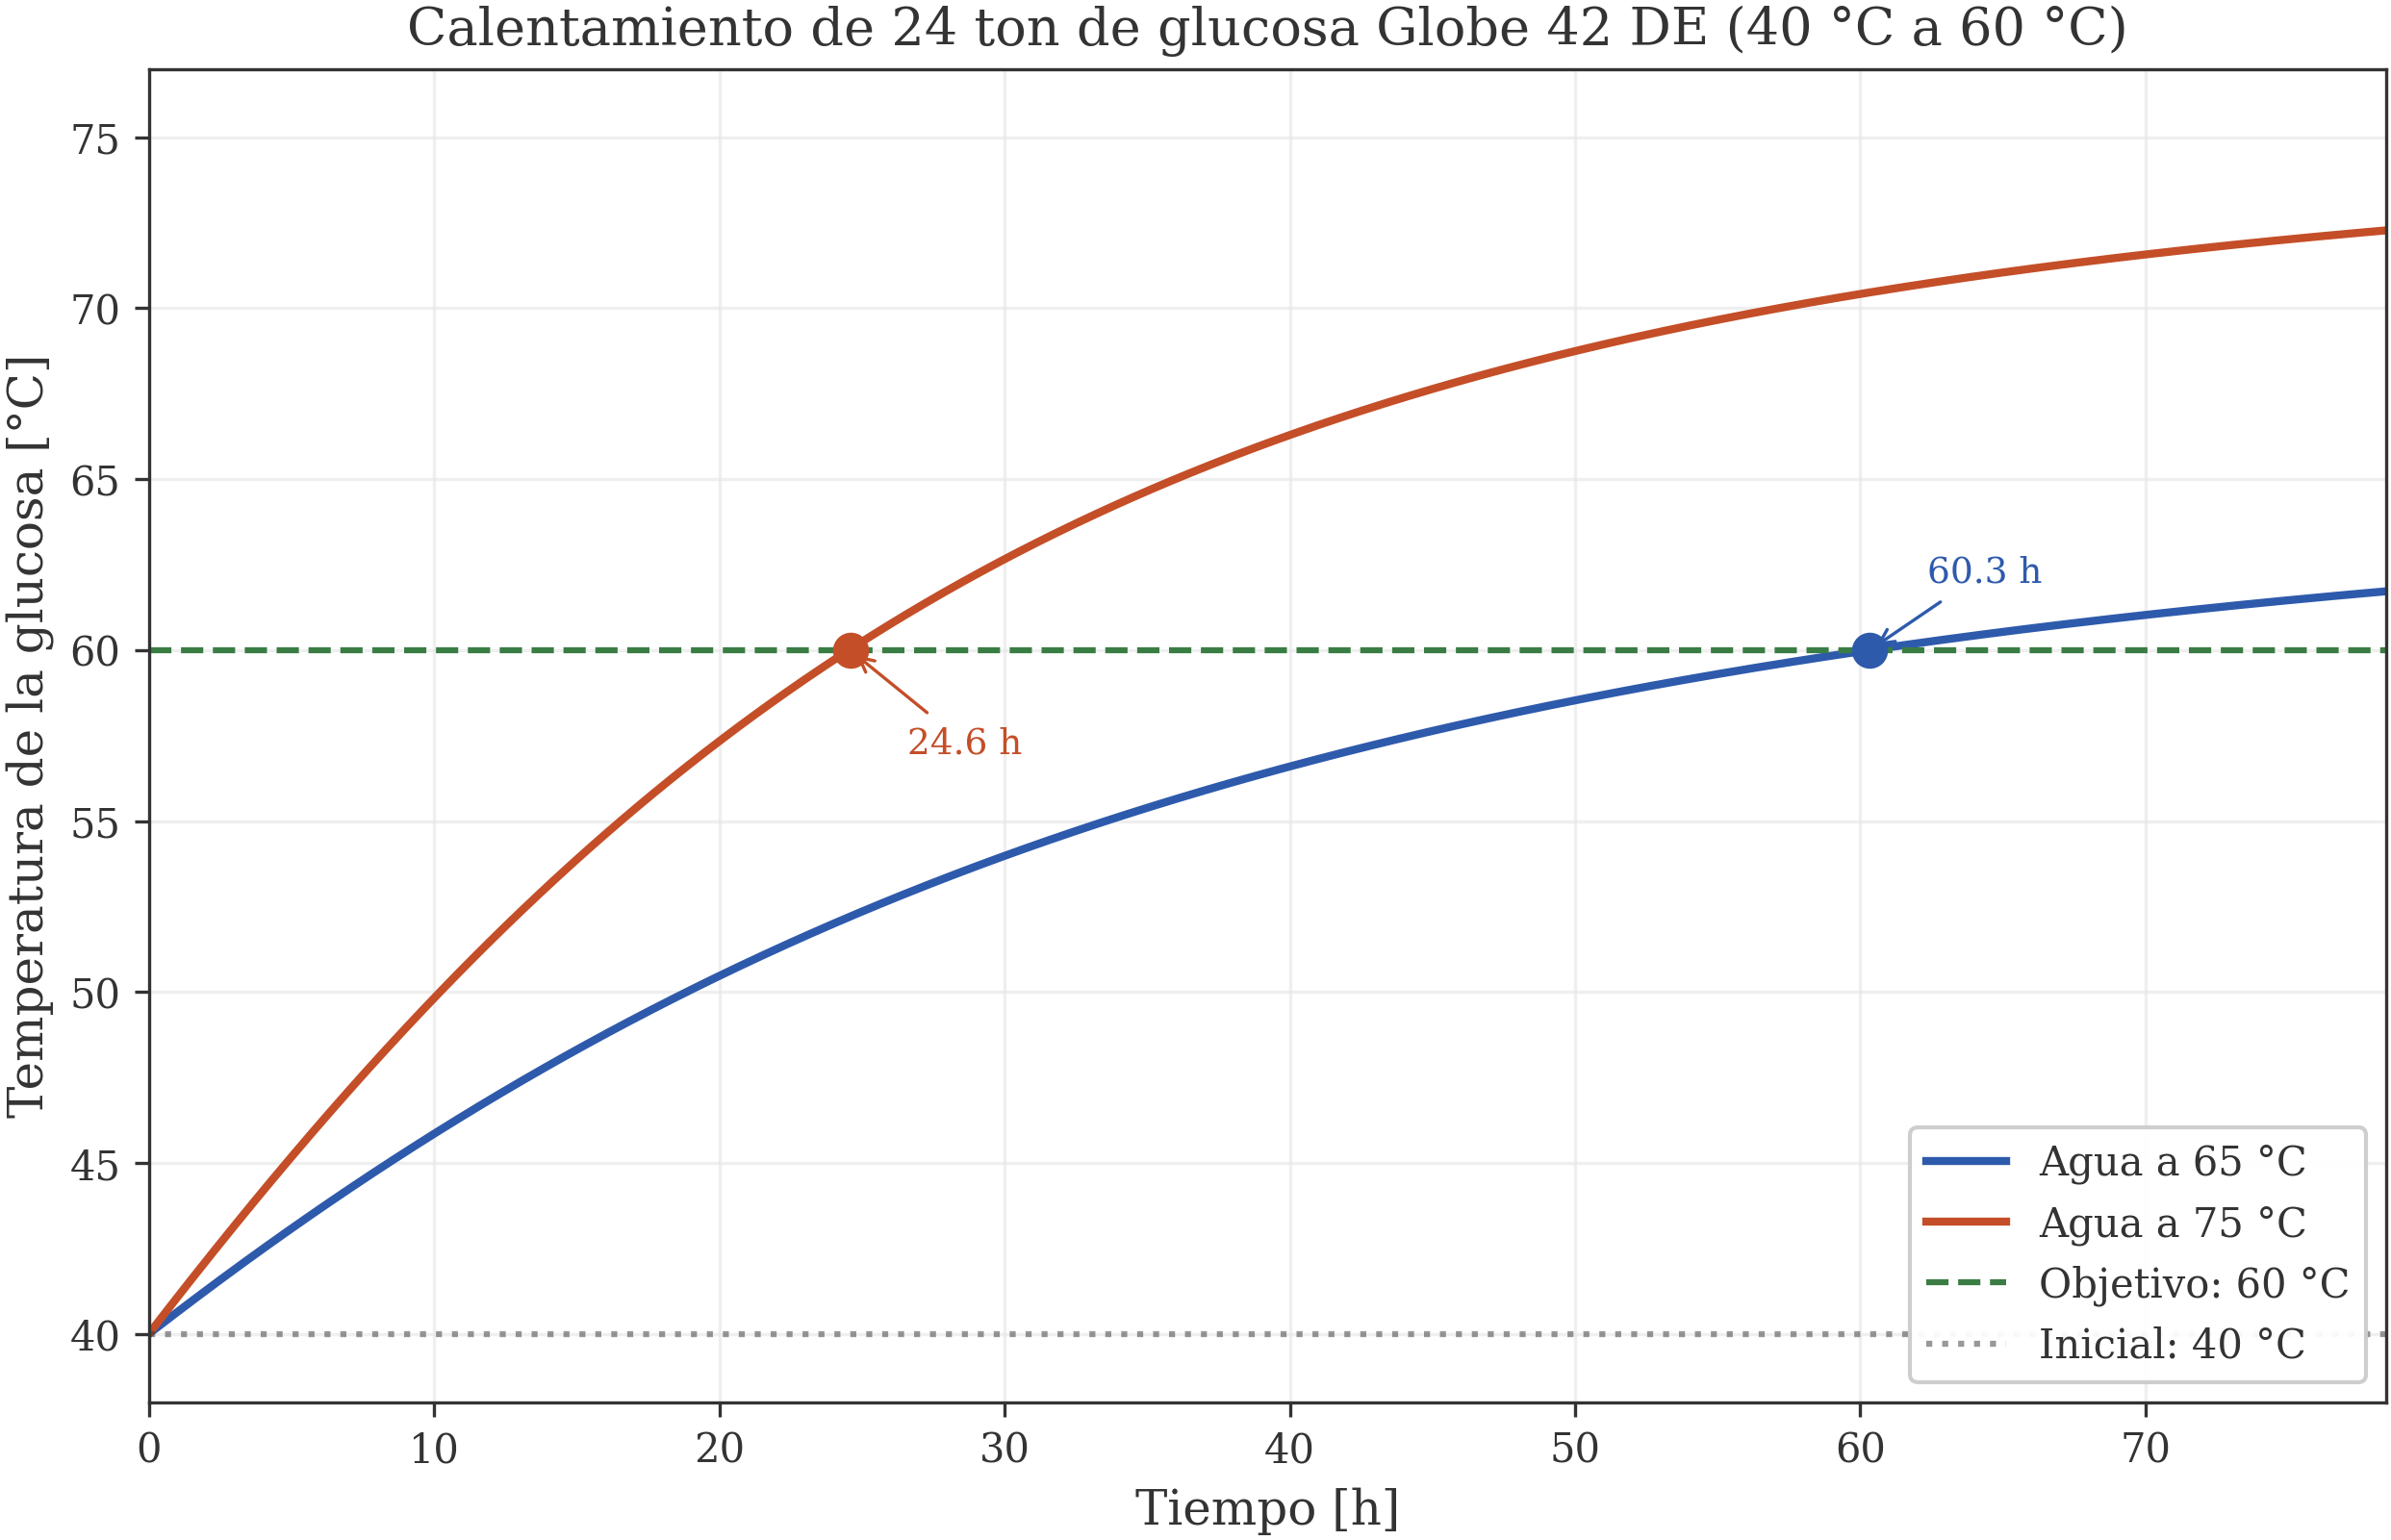
\includegraphics[width=0.85\textwidth]{../../results/figures/calentamiento_24ton_T_vs_t.pdf}
\caption{Curva de calentamiento de 24~ton de glucosa Globe 1130 desde 40~\textdegree C hasta 60~\textdegree C, con área de transferencia de 14~m\textsuperscript{2} y velocidad de agua de 2,5~m/s.}
\label{fig:calentamiento_24ton_T_vs_t}
\end{figure}

La Figura~\ref{fig:calentamiento_24ton_Q_vs_t} muestra el flujo de calor transferido a la glucosa en función del tiempo. El flujo de calor disminuye monótonamente a medida que se reduce la diferencia de temperatura entre el agua y la glucosa. El Escenario~B inicia con un flujo de 15,2~kW y finaliza cerca de 1,2~kW, mientras que el Escenario~A inicia en 9,1~kW.

\begin{figure}[H]
\centering
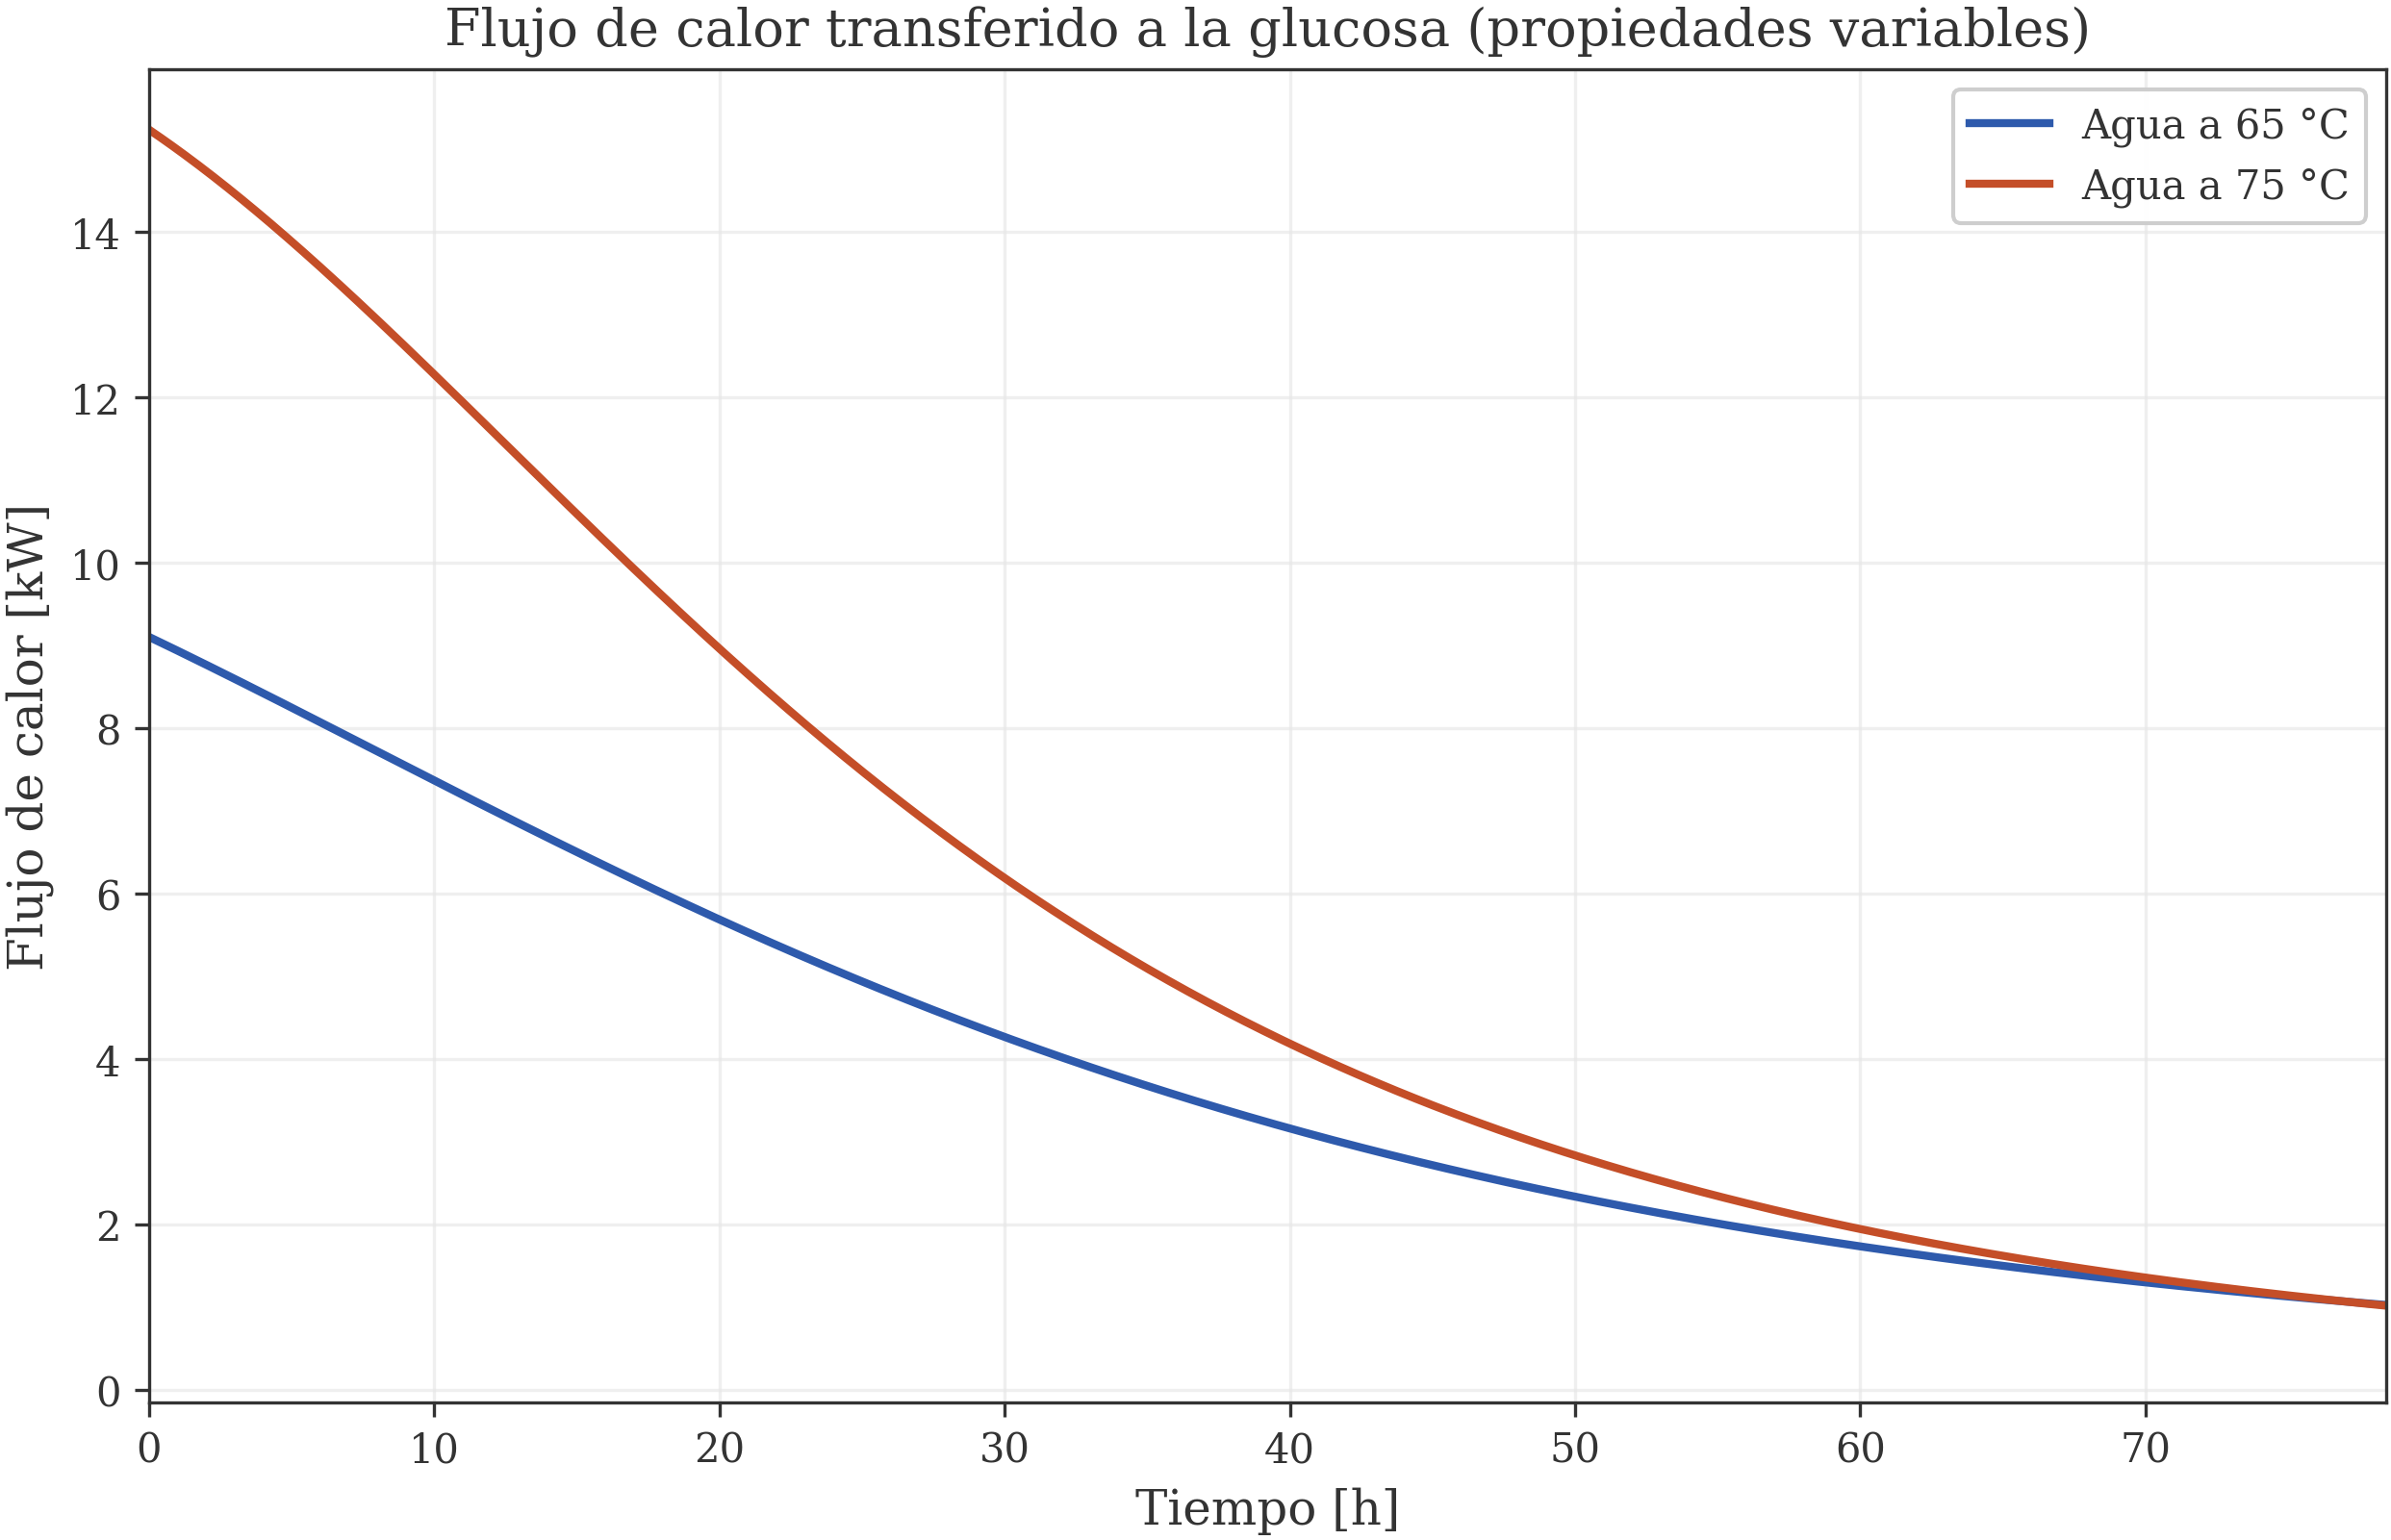
\includegraphics[width=0.85\textwidth]{../../results/figures/calentamiento_24ton_Q_vs_t.pdf}
\caption{Flujo de calor transferido a la glucosa durante el calentamiento, considerando propiedades termofísicas variables con la temperatura.}
\label{fig:calentamiento_24ton_Q_vs_t}
\end{figure}

La evolución del coeficiente global $U$ se presenta en la Figura~\ref{fig:calentamiento_24ton_U_vs_t}. Se observa el comportamiento no monótono descrito anteriormente, con un máximo en el Escenario~B de 36,2~W/(m\textsuperscript{2}$\cdot$\textdegree C) alrededor de los 20~h.

\begin{figure}[H]
\centering
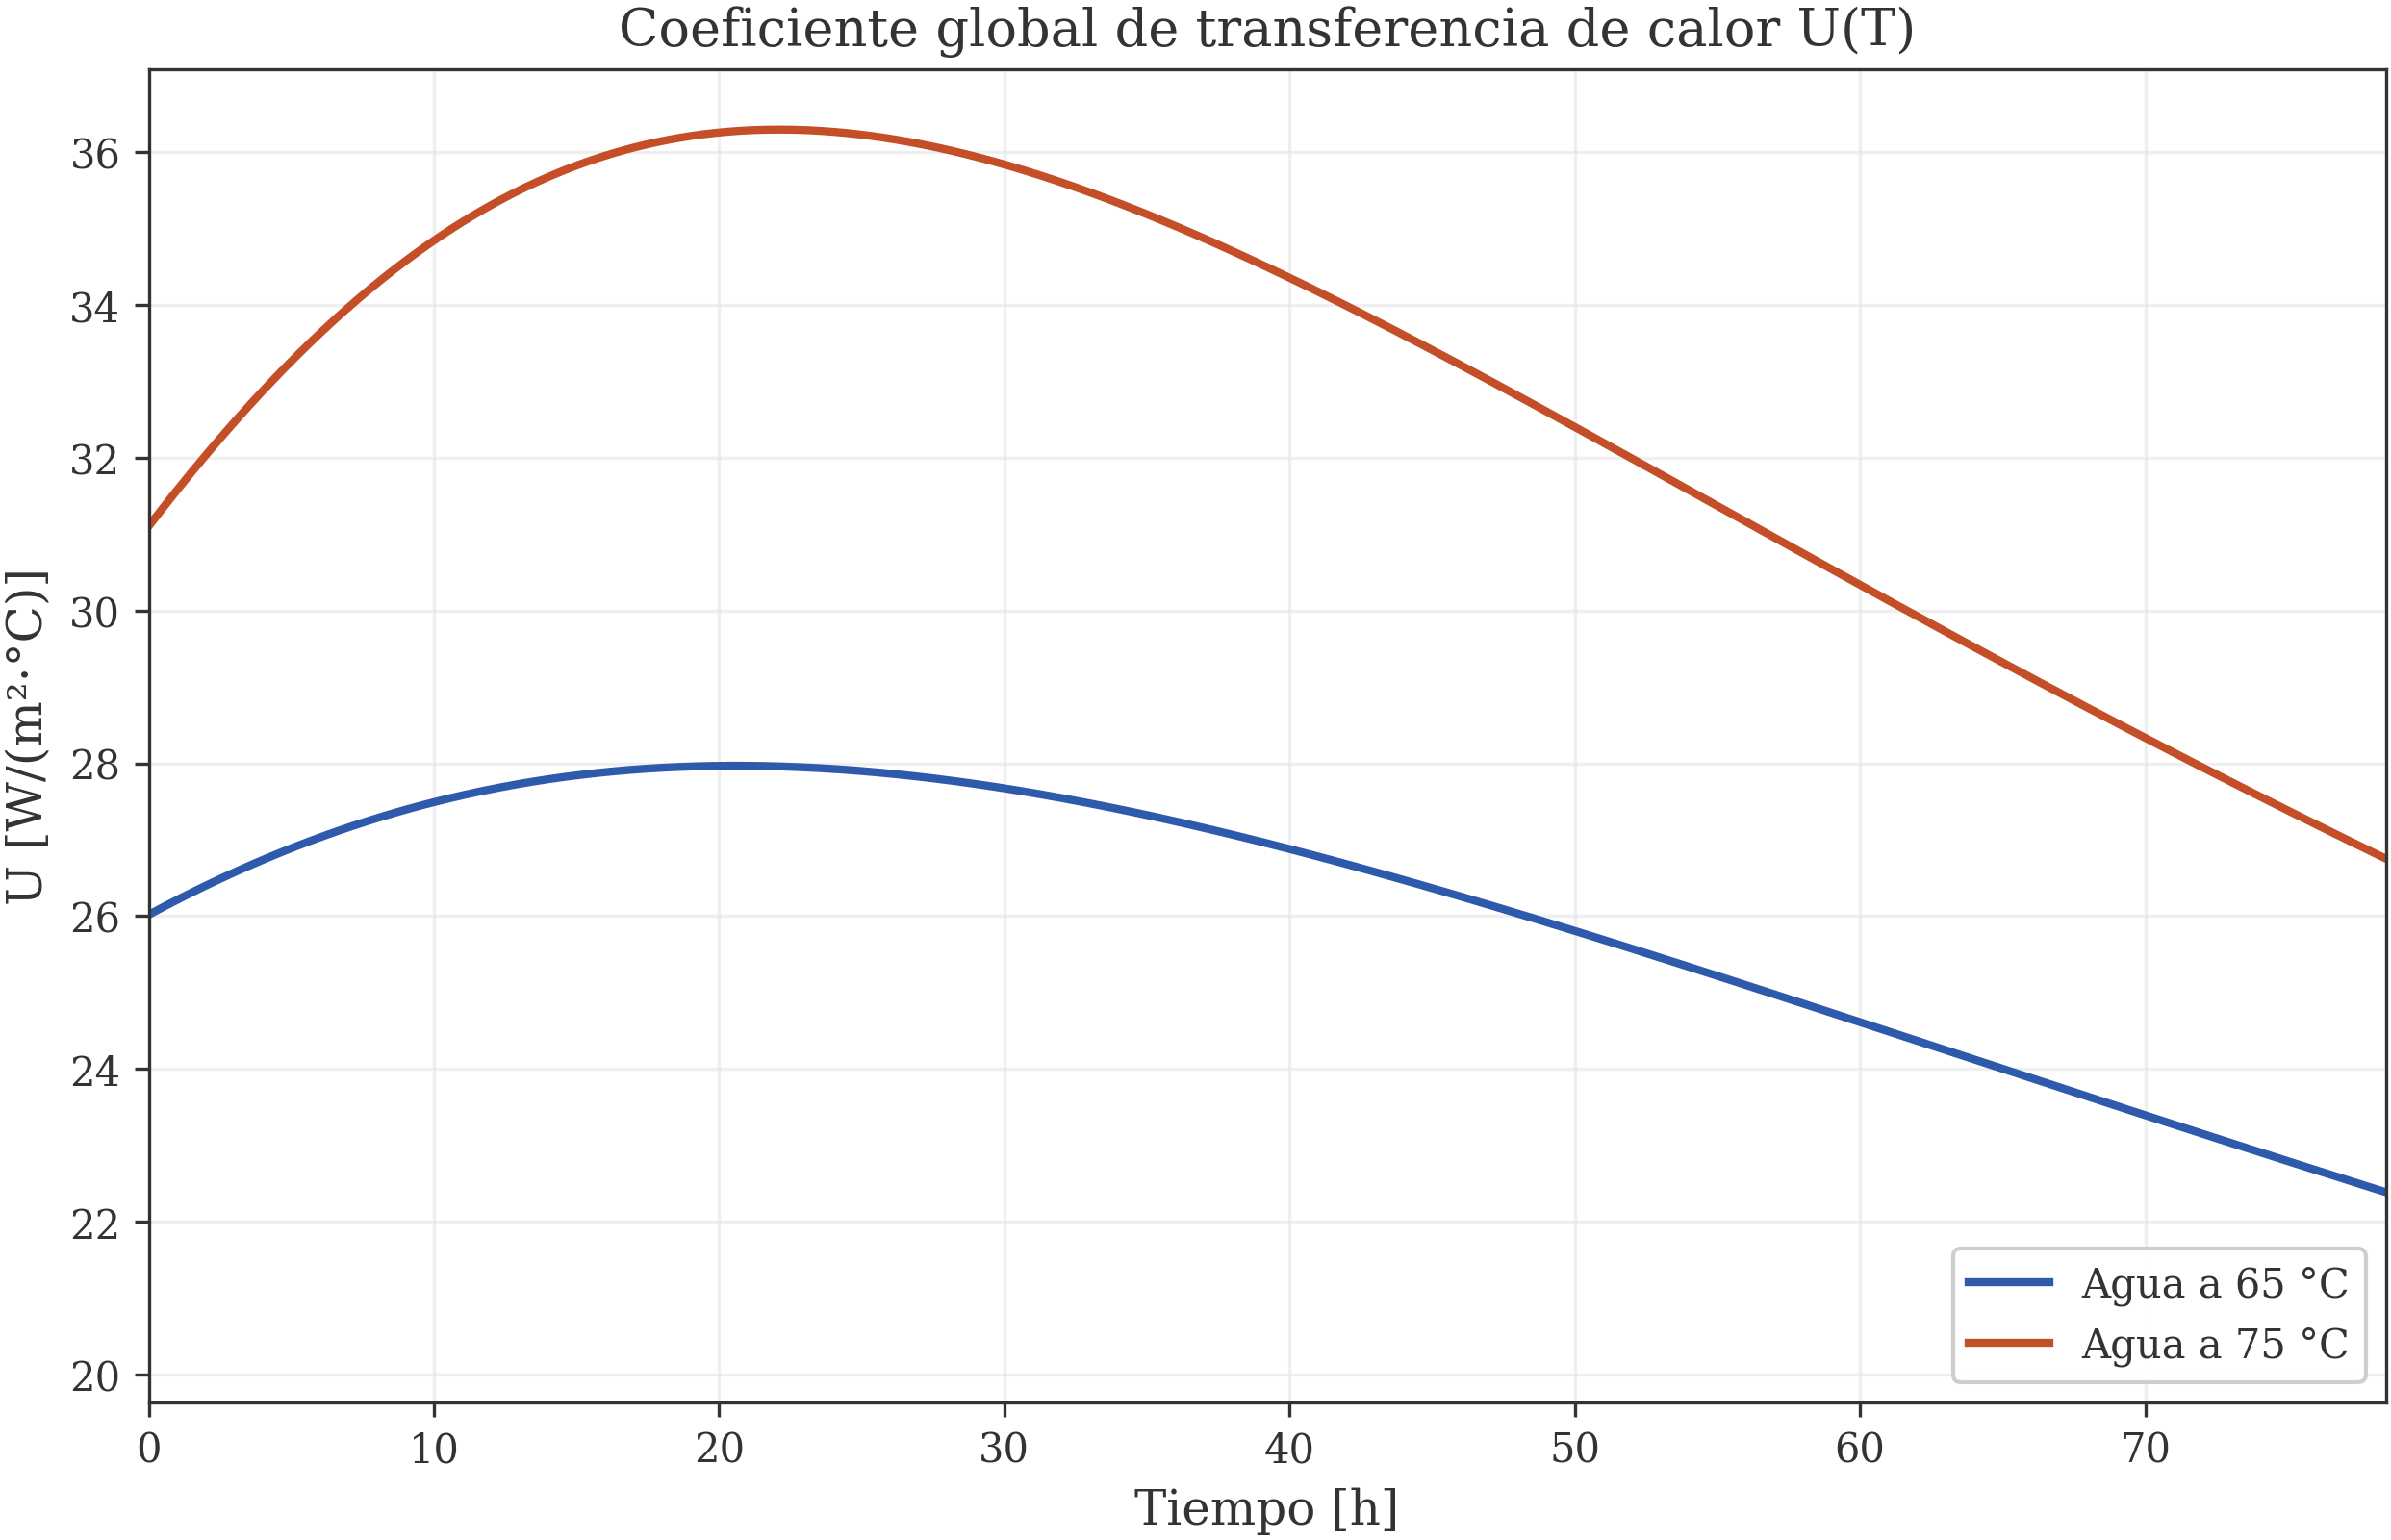
\includegraphics[width=0.85\textwidth]{../../results/figures/calentamiento_24ton_U_vs_t.pdf}
\caption{Coeficiente global de transferencia de calor en función del tiempo durante el calentamiento de 24~ton de glucosa.}
\label{fig:calentamiento_24ton_U_vs_t}
\end{figure}

La variación de las propiedades termofísicas en el rango de temperatura se ilustra en la Figura~\ref{fig:calentamiento_24ton_propiedades}. La viscosidad experimenta una caída de aproximadamente 6,5 veces, lo que explica la mejora inicial de $U$; sin embargo, el efecto de la temperatura de película sobre la convección natural limita el incremento posterior.

\begin{figure}[H]
\centering
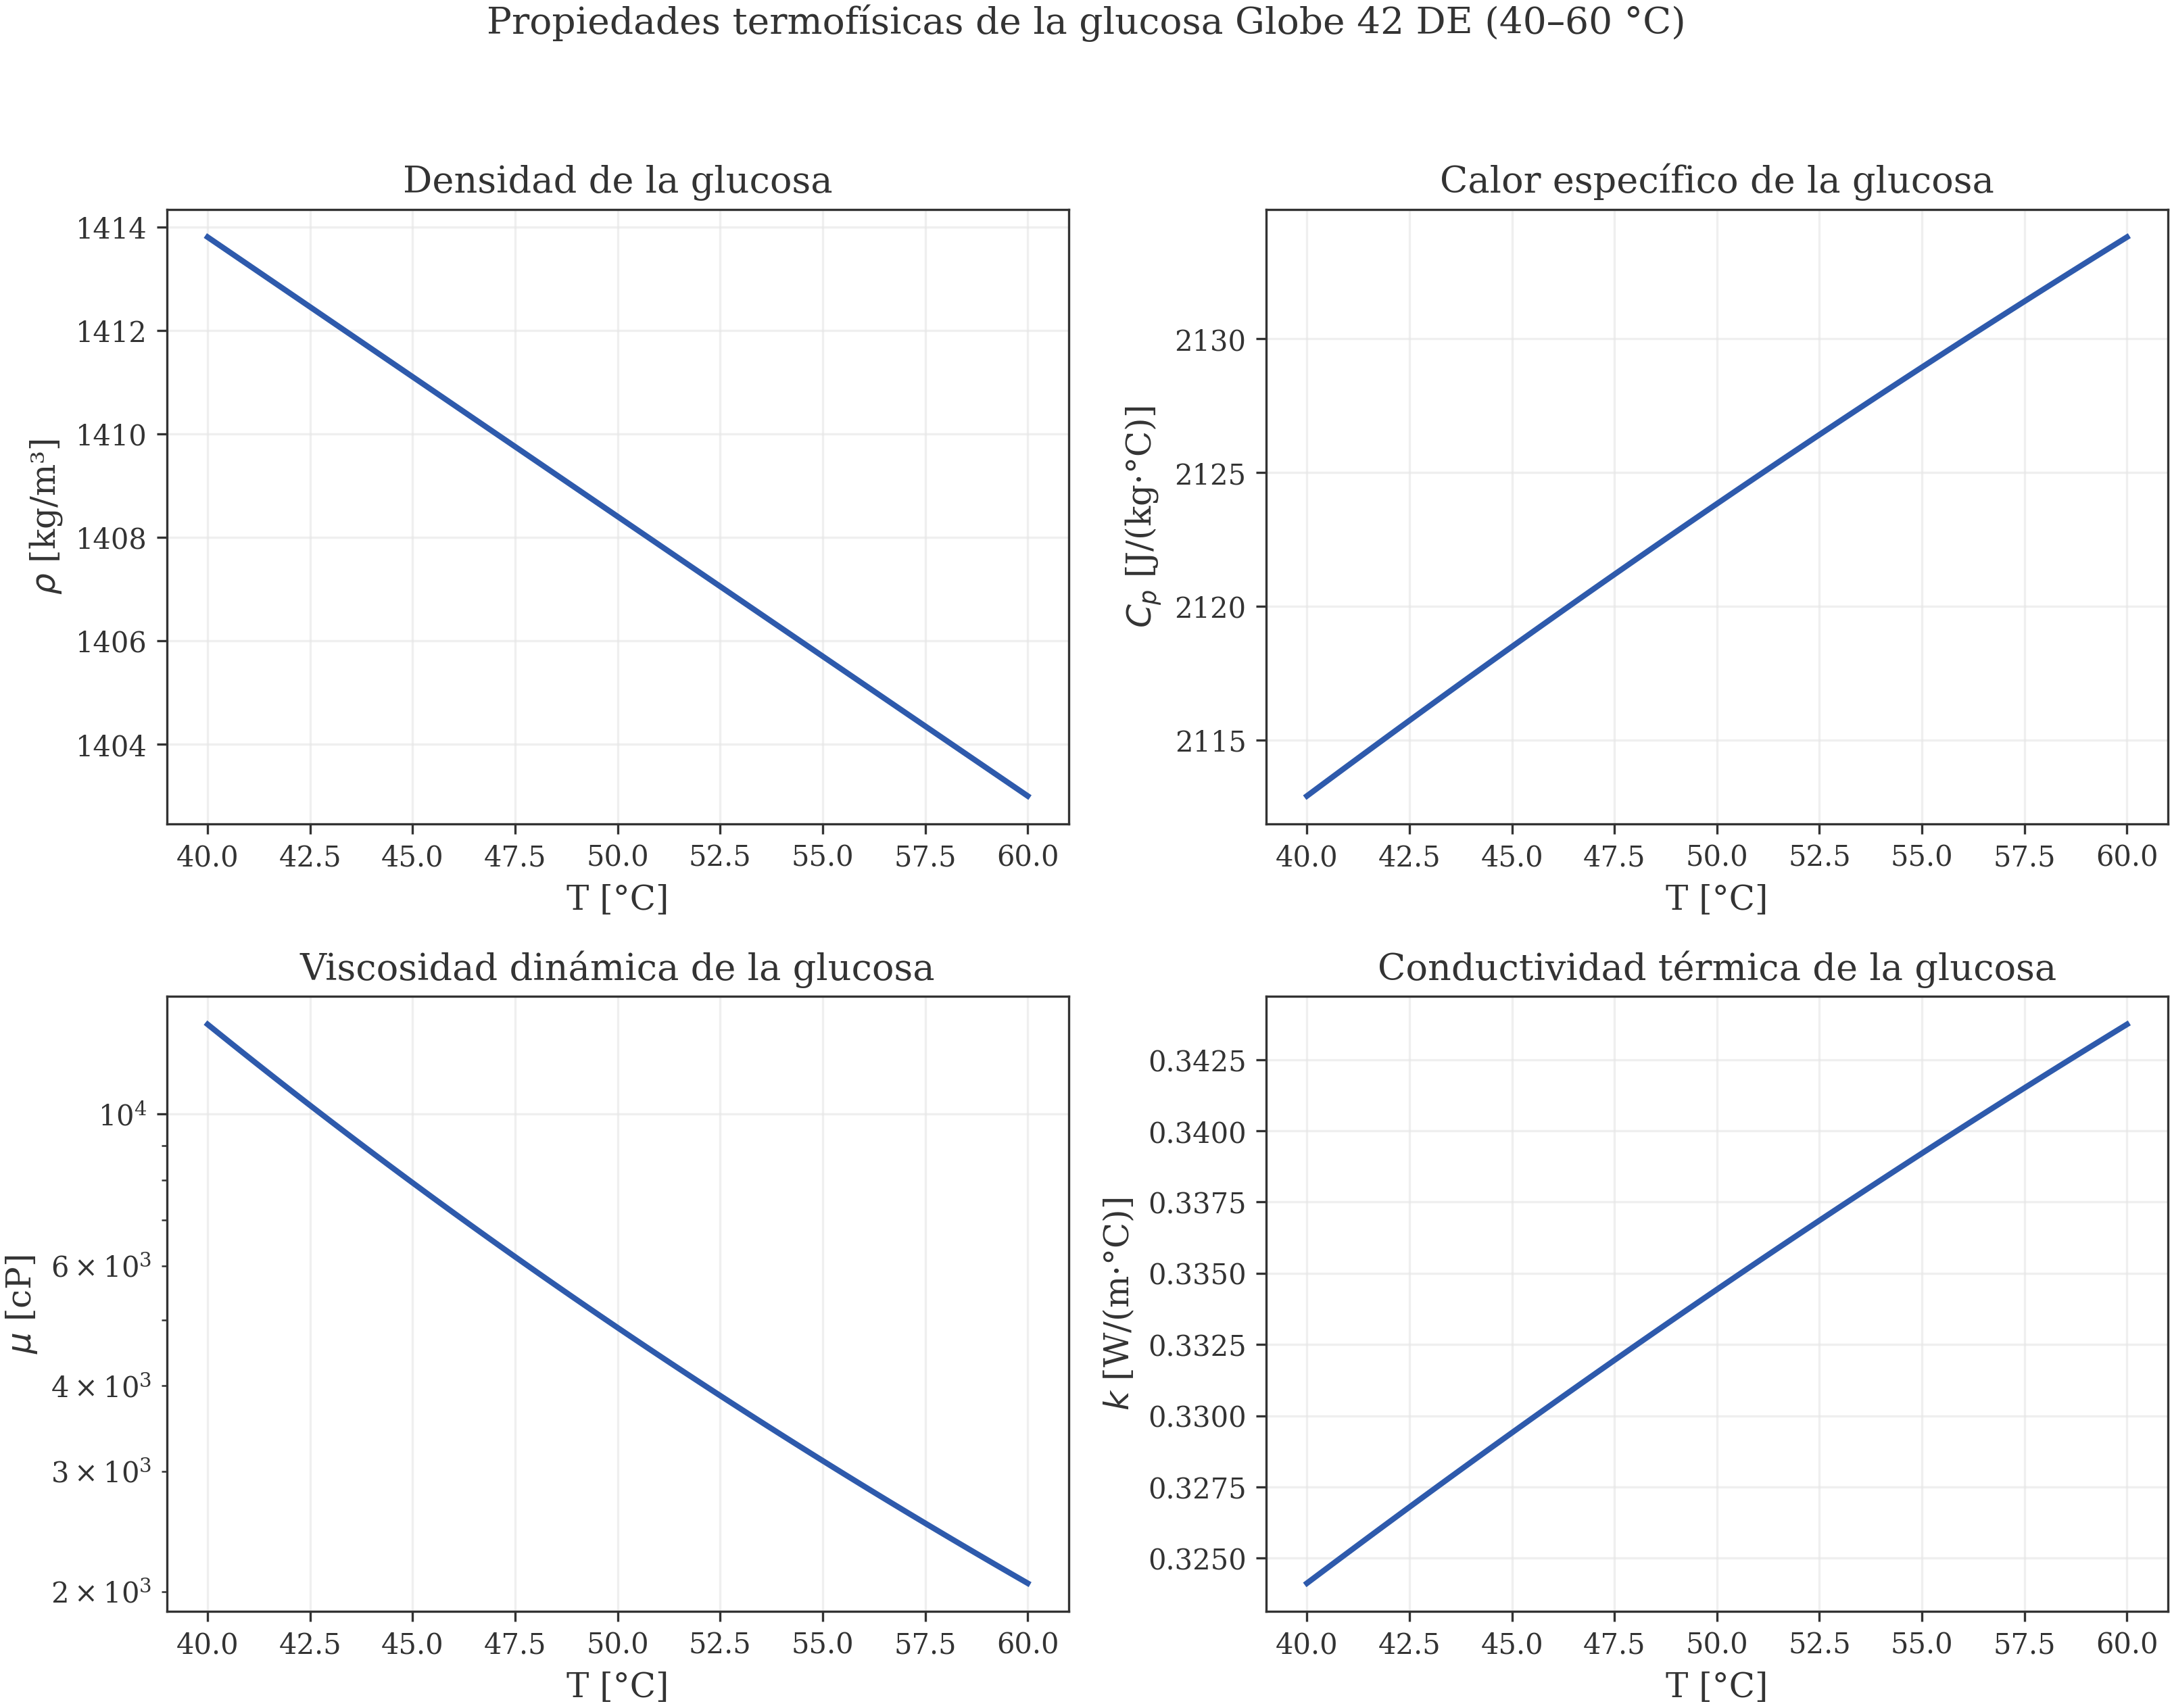
\includegraphics[width=0.95\textwidth]{../../results/figures/calentamiento_24ton_propiedades.pdf}
\caption{Propiedades termofísicas de la glucosa Globe 1130 en el rango de 40~\textdegree C a 60~\textdegree C: densidad, calor específico, viscosidad dinámica y conductividad térmica.}
\label{fig:calentamiento_24ton_propiedades}
\end{figure}

\subsection{Análisis de resultados}

Con el área de transferencia de 14~m\textsuperscript{2} se reduce el tiempo de calentamiento en una proporción directa, ya que el proceso está dominado por la resistencia del lado de la glucosa. Con agua a 75~\textdegree C, el sistema alcanza 60~\textdegree C en aproximadamente 24,6~h, lo cual resulta operativamente viable para un ciclo de preparación de carga. Con agua a 65~\textdegree C, el tiempo de 60,3~h supera el horizonte de una jornada operativa típica y requeriría programar el calentamiento con anticipación.

El flujo de calor máximo en el Escenario~B (15,2~kW) representa aproximadamente 1,7 veces el valor del Escenario~A (9,1~kW), mientras que la energía total transferida es prácticamente la misma en ambos casos porque depende exclusivamente de la masa y del cambio de temperatura. Esto indica que la temperatura del agua de calentamiento afecta principalmente la velocidad del proceso y no el consumo energético total.

\subsection{Extensión a niveles del 50~\% y 80~\% del tanque con pérdidas térmicas}

El análisis anterior ignora las pérdidas térmicas porque la masa de 24~ton se considera contenida en un recipiente independiente. Para evaluar el comportamiento real del tanque Tag~53A-90A-0056, se extiende el modelo al volumen operativo completo, incluyendo pérdidas al ambiente a través del área real expuesta (149,7~m\textsuperscript{2}) con aislamiento de lana mineral de 50,8~mm. El balance de energía se expresa como:

\begin{equation}
m_g \, C_{p,g}(T_g) \, \frac{dT_g}{dt} = U(T_g) \, A \, (T_w - T_g) - Q_{perd}(T_g)
\label{eq:balance_arranque_perdidas}
\end{equation}

donde $Q_{perd}(T_g)$ se calcula mediante el modelo de resistencias térmicas en serie descrito en la Sección~\ref{sec:metodologia_U}. El volumen total del tanque es 222,8~m\textsuperscript{3}; por tanto, el 50~\% equivale a 111,4~m\textsuperscript{3} y el 80~\% a 178,2~m\textsuperscript{3}. A 40~\textdegree C, las masas correspondientes son aproximadamente 157,5~ton y 252,0~ton.

La Tabla~\ref{tab:resultados_arranque_niveles} resume el comportamiento del sistema para ambos niveles y ambas temperaturas de agua, simulando hasta 96~h.

\begin{table}[H]
\centering
\caption{Resultados del calentamiento batch del tanque con pérdidas térmicas ($A = 14~\text{m}^2$, $v_w = 2{,}5~\text{m/s}$).}
\label{tab:resultados_arranque_niveles}
\begin{tabular}{@{}lcccc@{}}
\toprule
\textbf{Escenario} & \textbf{Nivel inicial} & \textbf{$T_w$ [\textdegree C]} & \textbf{$T$ a 96~h [\textdegree C]} & \textbf{Tiempo a 60~\textdegree C [h]} \\
\midrule
C & 80~\% & 65 & 44,27 & No alcanza en 96~h \\
D & 80~\% & 75 & 47,81 & No alcanza en 96~h \\
E & 50~\% & 65 & 46,31 & No alcanza en 96~h \\
F & 50~\% & 75 & 51,50 & No alcanza en 96~h \\
\bottomrule
\end{tabular}
\end{table}

Ninguno de los cuatro escenarios alcanza 60~\textdegree C dentro de las 96~h simuladas. La inercia térmica de la masa de glucosa, combinada con pérdidas de aproximadamente 14,7~MJ/h a 60~\textdegree C, hace que el aporte de la chaqueta de 14~m\textsuperscript{2} sea insuficiente para elevar la temperatura del contenido total del tanque en horizontes operativos razonables. El Escenario~F (50~\%, 75~\textdegree C) muestra la mayor aproximación, alcanzando 51,50~\textdegree C a las 96~h.

La Figura~\ref{fig:arranque_T_vs_t_comparativa} compara las curvas de temperatura para los seis escenarios evaluados: 24~ton sin pérdidas, 50~\% con pérdidas y 80~\% con pérdidas, para agua a 65~\textdegree C y 75~\textdegree C.

\begin{figure}[H]
\centering
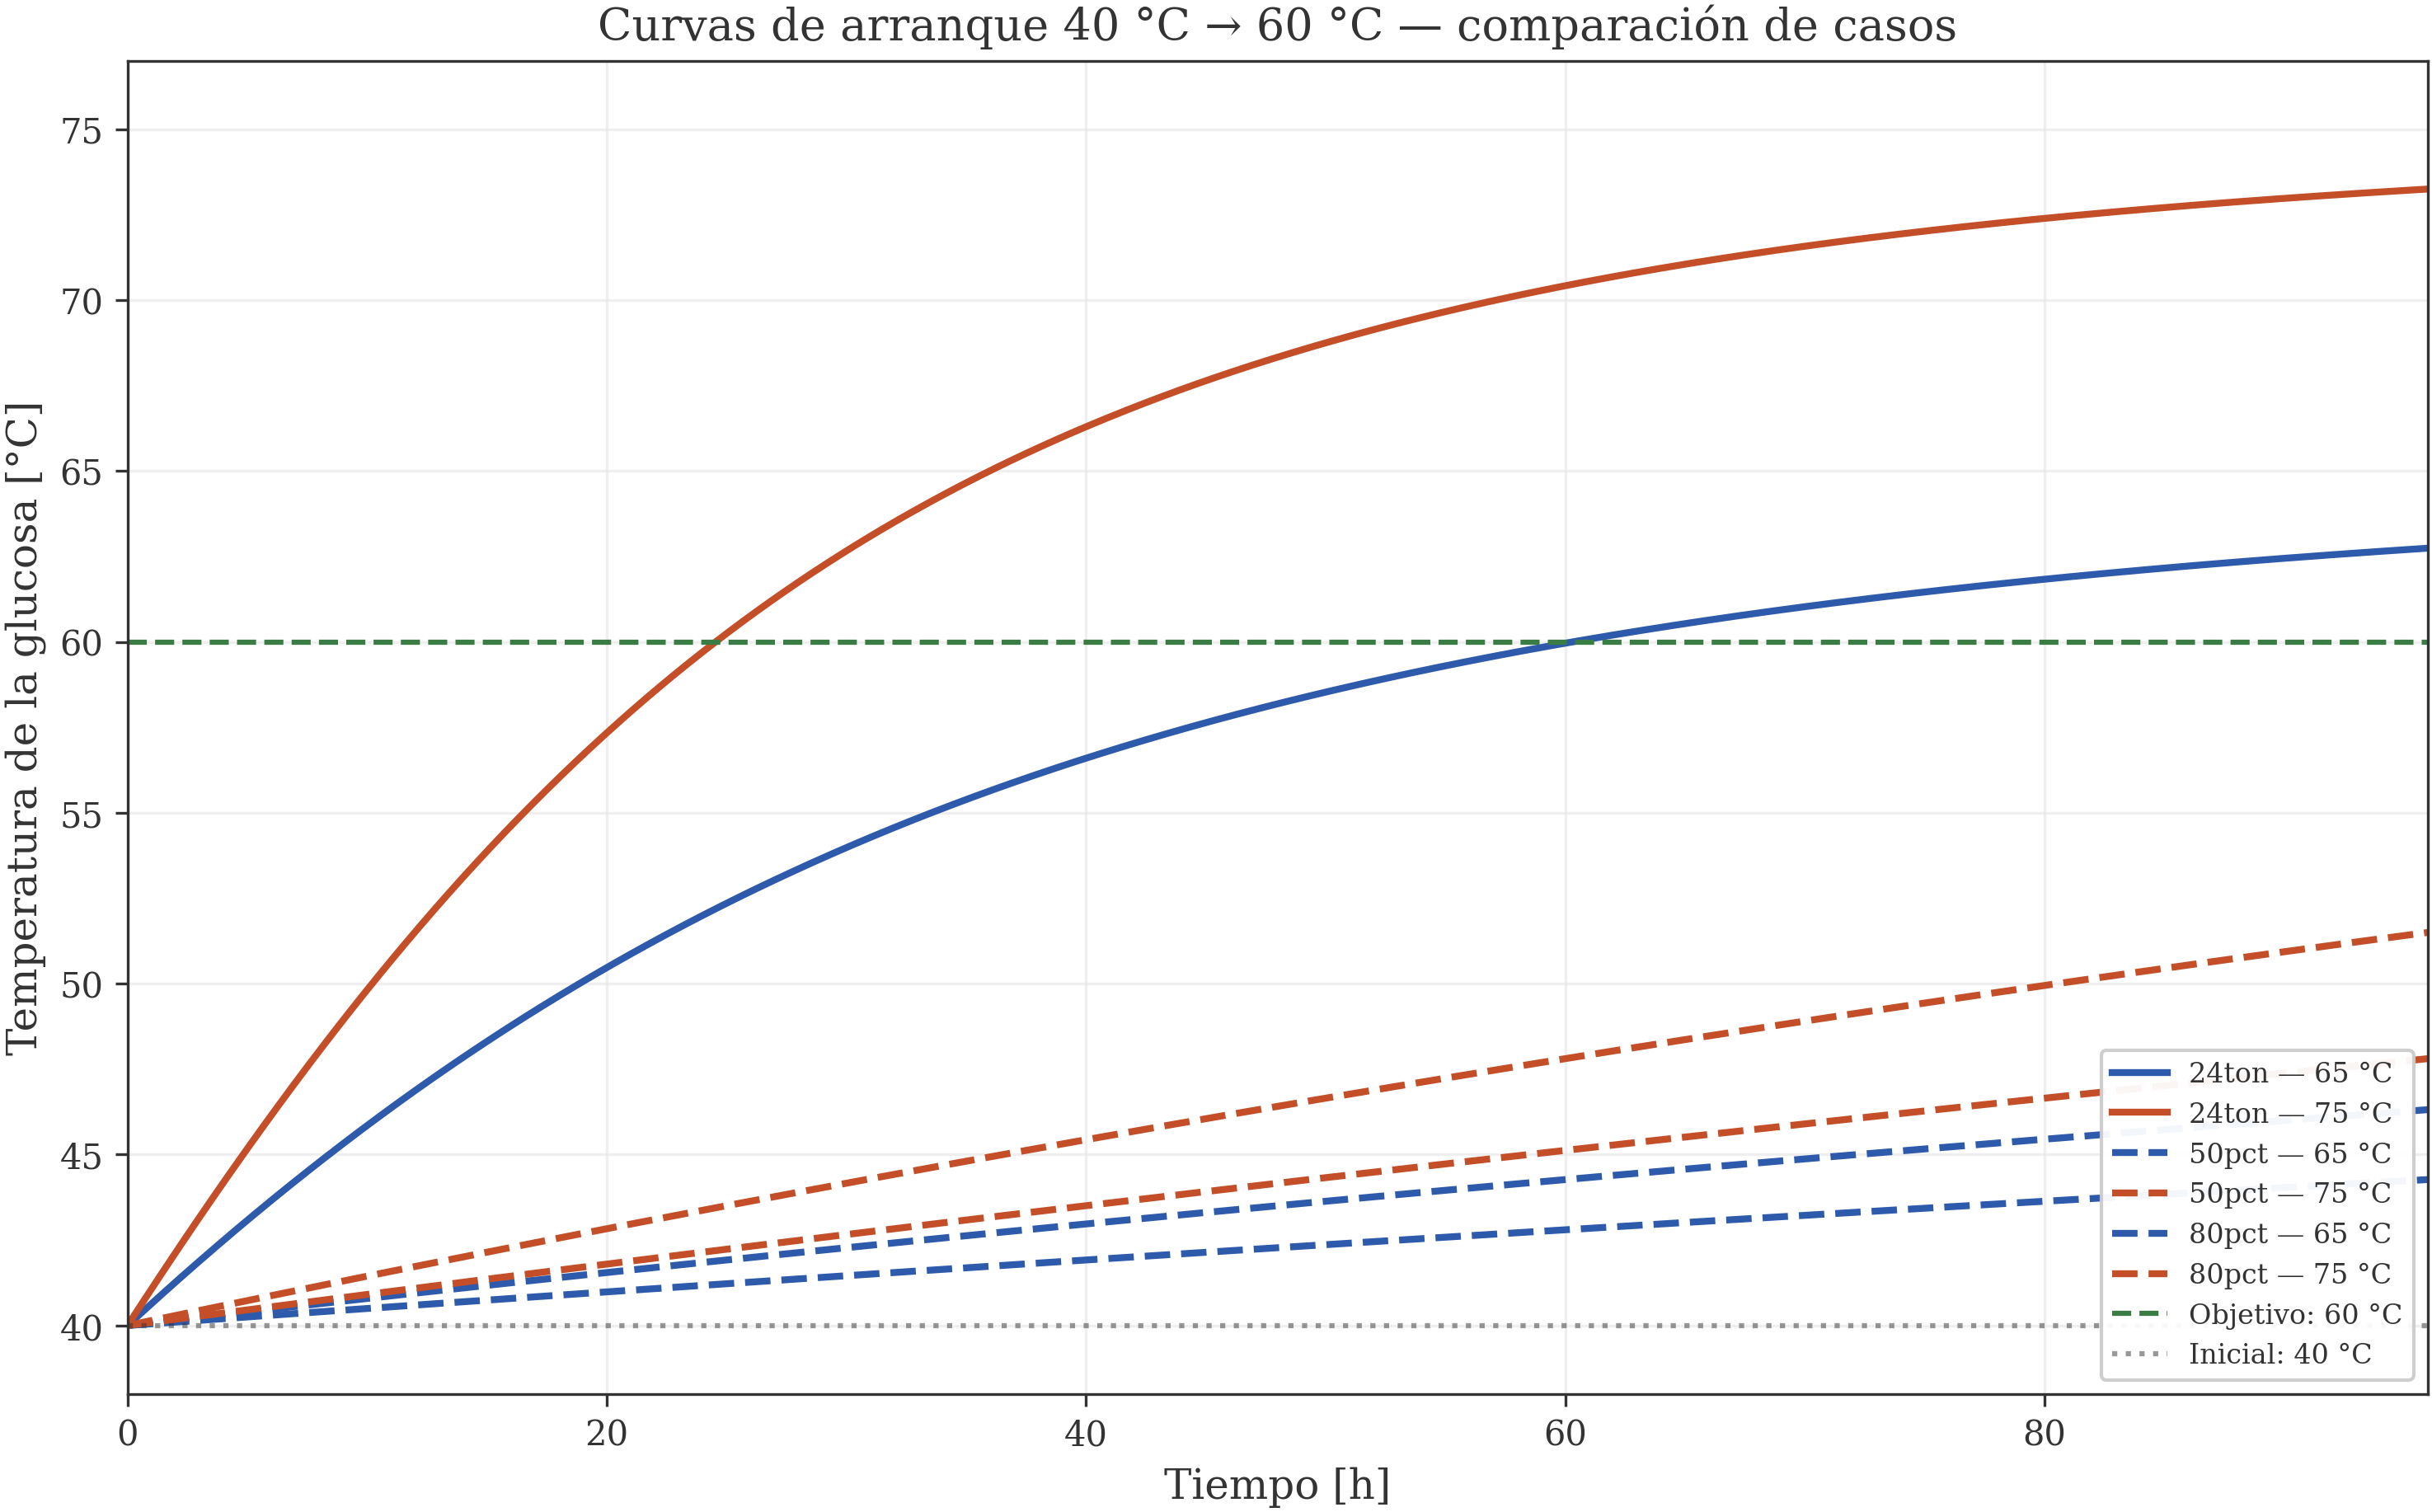
\includegraphics[width=0.95\textwidth]{../../results/figures/curva_arranque_T_vs_t_comparativa.pdf}
\caption{Comparativa de curvas de calentamiento batch para 24~ton (sin pérdidas), 50~\% y 80~\% del tanque (con pérdidas térmicas reales).}
\label{fig:arranque_T_vs_t_comparativa}
\end{figure}

La Figura~\ref{fig:arranque_por_caso} presenta las curvas individuales de temperatura y flujo de calor para cada caso, destacando el efecto del término de pérdidas sobre la asintota térmica del sistema.

\begin{figure}[H]
\centering
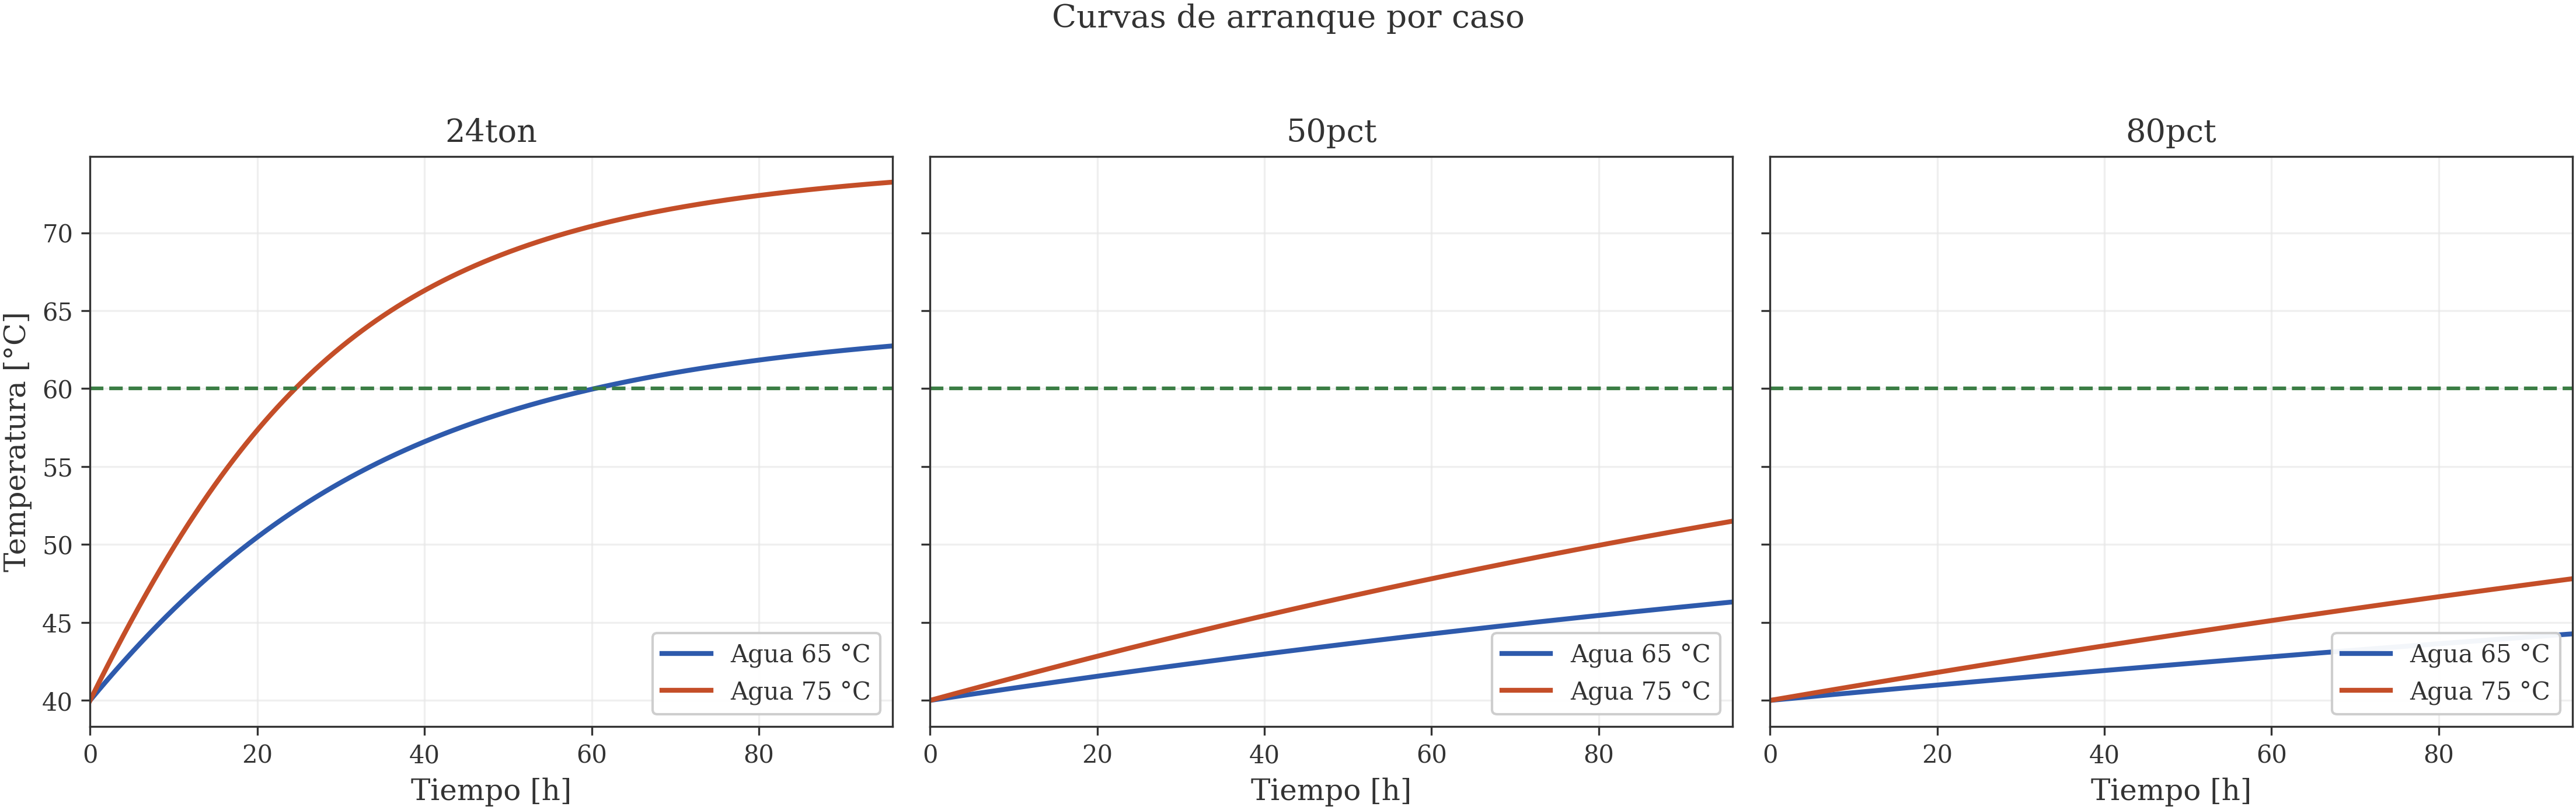
\includegraphics[width=0.95\textwidth]{../../results/figures/curva_arranque_por_caso.pdf}
\caption{Curvas individuales de temperatura y flujo de calor por escenario de arranque.}
\label{fig:arranque_por_caso}
\end{figure}

\subsection{Interpretación de los resultados de arranque}

El caso de 24~ton sin pérdidas representa una condición idealizada que sirve para dimensionar el área mínima necesaria para calentar una carga aislada en un tiempo aceptable. En cambio, los escenarios de 50~\% y 80~\% del tanque incluyen la realidad de las pérdidas térmicas y la gran inercia del volumen operativo. La diferencia cualitativa es clara: mientras que el sistema de 24~ton evoluciona hacia la temperatura del agua de calentamiento, el sistema real del tanque alcanza una temperatura de equilibrio mucho menor porque el aporte térmico no compensa las pérdidas cuando la diferencia de temperatura con el ambiente crece.

Estos resultados indican que el arranque del tanque completo desde 40~\textdegree C hasta 60~\textdegree C con una chaqueta de 14~m\textsuperscript{2} no es viable en un horizonte de días. Para alcanzar 60~\textdegree C en todo el contenido del tanque se requeriría aumentar el área de transferencia, elevar la temperatura del agua de calentamiento o reducir las pérdidas térmicas mediante un aislamiento adicional. La estrategia operativa recomendada consiste en calentar primero un volumen reducido equivalente a una descarga (24~ton) y luego iniciar el ciclo de recarga y descarga descrito en la Sección~\ref{sec:ciclo_12m3h}.
